\chapter{Πειραματικά αποτελέσματα}
\section{Περιγραφή πειραμάτων}
Στόχος της παρούσας ενότητας είναι ο έλεγχος του συστήματος Automated Data Scientist, καθώς και της συνεισφοράς των τεχνικών που εφαρμόσαμε και περιγράψαμε στην ενότητα \ref{sec:techniques}. Προς αυτό το σκοπό σχεδιάσαμε τα ακόλουθα πειράματα, τα οποία θα αναλύσουμε στη συνέχεια:
\begin{itemize}
	\item αξιολόγηση των HPP μοντέλων
	\item αξιολόγηση του ensemble με προς-τα-εμπρός επιλογή μοντέλων
	\item συνολική αξιολόγηση του συστήματος
\end{itemize}

\paragraph{Περιγραφή σετ δεδομένων} Για τη διεξαγωγή των πειραμάτων συλλέξαμε ένα πλήθος 123 σετ δεδομένων από διάφορες πηγές. (Στο παράρτημα \ref{appendix:Datasets} βρίσκεται ένας λεπτομερής κατάλογος περιγραφής τους.) Άξονας αναζήτησης κατά τη συλλογή ήταν η εύρεση σετ δεδομένων δυαδικής ταξινόμησης με ετερογενή χαρακτηριστικά, ώστε ο έλεγχος του συστήματος να είναι αντιπροσωπευτικός για το πραγματικό πλήθος σετ δεδομένων. Προκειμένου να υπάρχει μία κοινή διεπαφή για τα πειράματα ήταν απαραίτητος ο "καθαρισμός" των σετ δεδομένων μέσω των ακόλουθων βημάτων:
\begin{itemize}
	\item μετατροπή αρχείων σε comma-delimited .csv. Τα πηγαία αρχεία βρίσκονταν σε μορφές .csv, .txt, .xlsx, .arff και .mysql.
	\item καθορισμός κλάσης. Στη πλειοψηφία των περιπτώσεων η κλάση αναγνωριζόταν χειροκίνητα από την περιγραφή του σετ δεδομένων. Συλλέχθηκαν και σετ δεδομένων που ήταν πολλαπλής ταξινόμησης και παλινδρόμησης. Στην πρώτη περίπτωση έγινε αντιστοίχηση σε δύο ουσιώδεις κλάσεις, ενώ στη δεύτερη βρέθηκε η μέση τιμή της μεταβλητής κλάσης και χρησιμοποιήθηκε ως κατώφλι για το διαχωρισμό των παραδειγμάτων σε δύο κλάσεις.
	\item αναγνώριση άγνωστων τιμών. Στα αρχεία που περιείχαν άγνωστες τιμές χρησιμοποιούνταν διάφοροι συμβολισμοί ("?", "*", "") οι οποίοι αντικαταστάθηκαν από κενά, ώστε να αναγνωρίζονται από την R ως NAs (Not Available).  
\end{itemize}
\section{Αξιολόγηση της τεχνικής βελτιστοποίησης υπερ-παραμέτρων με μετα-μάθηση και χρήση διαστημάτων πρόβλεψης}
Όπως είδαμε στην ενότητα \ref{sec:HPP} προϊόντα αυτής της τεχνικής είναι τα \gls{HPP} μοντέλα, καθένα εκ των οποίων έχει εκπαιδευτεί στη πρόβλεψη μίας υπερ-παραμέτρου ενός αλγορίθμου μηχανικής μάθησης. Σε αυτό το σημείο θα αξιολογήσουμε τα μοντέλα αυτά ως προς το σκοπό τους, δηλαδή πόσο καλά προβλέπουν τις βελτιστοποιημένες υπερ-παραμέτρους. Επίσης, θα σχολιάσουμε τη συνεισφορά της χρήσης διαστημάτων πρόβλεψης.

Για την παραγωγή των σετ μετα-δεδομένων, τα οποία χρησιμοποιούνται για την εκπαίδευση των HPP μοντέλων, είναι απαραίτητα δύο στάδια:
\begin{itemize}
	\item Εξαγωγή των μετα-χαρακτηριστικών κάθε σετ δεδομένων. Τα  81 μετα-χαρακτηριστικά που χρησιμοποιήσαμε περιγράφονται στον Πίνακα \ref{table:meta} και υπολογίστηκαν με χρήση του πακέτου mf\-Extractor του συστήματός μας. Βασίστηκαν σε εκτεταμένη βιβλιογραφική έρευνα και προσπαθούν να συμπεριλάβουν όλα τα είδη μετα-χαρακτηριστικών που εμφανίζονται σε παρόμοιες εργασίες.Πριν τον υπολογισμό τους έγινε μετατροπή των κατηγορικών χαρακτηριστικών σε μεταβλητές-δείκτες, ώστε να υπάρχει ομοιόμορφη αντιμετώπιση.   
	 \begin{table}[!htb]
	 	\footnotesize
	 	\begin{center}
	 	\caption{Λίστα μετα-χαρακτηριστικών, τα οποία χρησιμοποιήθηκαν για την εκπαίδευση των HPP μοντέλων}
	 	\label{table:meta}
	 		\begin{tabular}{ |l l l | } 
	 			\hline
	 			\multicolumn{3}{|c|}{Μετα-χαρακτηριστικά}    \\
	 			\hline
	 			\textbf{Απλά} & \textbf{Θεωρίας Πληροφορίας} &   \textbf{Στατιστικά Kατηγορικά}  \\
	 			Πλήθος χαρακτηριστικών & Εντροπία Κλάσης  &   Πλήθος επιπέδων \\
	 			Λογάριθμος πλήθους χαρακτηριστικών &    & \\
	 			Πλήθος παραδειγμάτων &  \textbf{Στατιστικά Aριθμητικά} & \textbf{Μετα2-}   \\
	 			Λογάριθμος πλήθους παραδειγμάτων & Άθροισμα & Άθροισμα     \\
	 			Πλήθος χαρακτηριστικών με άγνωστες τιμές & Μέση τιμή & Μέση τιμή  \\
	 			Ποσοστό πλήθους χαρακτηριστικών με άγνωστες τιμές & Τυπική απόκλιση & Τυπική απόκλιση   \\
	 			Πλήθος παραδειγμάτων με άγνωστες τιμές & Ελάχιστη τιμή & Ελάχιστη τιμή    \\
	 			Ποσοστό πλήθους παραδειγμάτων με άγνωστες τιμές & Μέγιστη τιμή & Μέγιστη τιμή   \\
	 			Πλήθος άγνωστων τιμών & Κυρτότητα & Κυρτότητα  \\
	 			Λογάριθμος πλήθους άγνωστων τιμών & Λοξότητα & Λοξότητα \\
	 			Πλήθος αριθμητικών χαρακτηριστικών & Ποσοστό \gls{PC}s για $95\%$ διακύμανση & \\
	 			Πλήθος κατηγορικών χαρακτηριστικών &  Κυρτότητα πρώτης \gls{PC}& \\
	 			Πιθανότητες κλάσης & Λοξότητα πρώτης \gls{PC}& \\
	 			Ελάχιστη πιθανότητα κλάσης & &   \\
                Μέγιστη πιθανότητα κλάσης & &  \\
                Μέση τιμή πιθανοτήτων κλάσης & &  \\
                Τυπική απόκλιση πιθανοτήτων κλάσης &  & \\
                \hline
	 		\end{tabular}    
	 	\end{center}
	 \end{table}
	
	Καθώς το πλήθος των μετα-χαρακτηριστικών είναι δυσανάλογο των διαθέσιμων σετ δεδομένων για εκπαίδευση των \gls{HPP} μοντέλων, θα επιστρατευθούν τεχνικές επιλογής των βέλτιστων. Σε πρώτη φάση αφαιρέσαμε τα γραμμικά συσχετισμένα χαρακτηριστικά, όπως αυτά υπολογίστηκαν στο σετ δεδομένων εκπαίδευσης, οπότε η τελική λίστα προέκυψε:
	 \begin{table}[!htb]
	 	\footnotesize
	 	\begin{center}
	 		\caption{Λίστα μετα-χαρακτηριστικών μετά από εφαρμογή φιλτραρίσματος}
	 		\label{table:meta}
	 		\begin{tabular}{ |l l| } 
	 			\hline
	 		     Άθροισμα αθροισμάτων & Τυπική απόκλιση επιπέδων    \\
	 			Άθροισμα μέγιστων τιμών &  Κυρτότητα επιπέδων  \\
	 			Μέση τιμή τυπικών αποκλίσεων  & Λοξότητα επιπέδων    \\
	 		    Μέση τιμή ελαχίστων τιμών &  Πλήθος χαρακτηριστικών  \\
	 			Μέση τιμή κυρτοτήτων &   Λογάριθμος πλήθους χαρακτηριστικών \\
	 			Μέση τιμή λοξοτήτων &    Πλήθος παραδειγμάτων\\
	 			Τυπική απόκλιση ελαχίστων τιμών & Λογάριθμος πλήθους παραδειγμάτων   \\
	 			Ελάχιστη τιμή μέσων τιμών &  Ποσοστό αγνώστων τιμών  \\
	 			Ελάχιστη τιμή τυπικών αποκλίσεων &  Πλήθος αριθμητικών χαρακτηριστικών  \\
	 			Ελάχιστη τιμή ελαχίστων τιμών &  Πλήθος κατηγορικών χαρακτηριστικών  \\
	 			Ελάχιστη τιμή μεγίστων τιμών &  Μέγιστη πιθανότητα κλάσης    \\
	 			Ελάχιστη τιμή λοξοτήτων & Μέση τιμή πιθανοτήτων κλάσης   \\
	 			Κυρτότητα ελαχίστων τιμών & Ποσοστό \gls{PC} για $95\%$ διακύμανση  \\
	 			Κυρτότητα μεγίστων τιμών & Κυρτότητα πρώτης \gls{PC}   \\
	 			Λοξότητα λοξοτήτων & Λοξότητα \gls{PC}   \\
	 		    Άθροισμα επιπέδων &    \\
	 			\hline
	 		\end{tabular}    
	 	\end{center}
	 \end{table}
	\FloatBarrier
	\item Εύρεση των βέλτιστων υπερ-παραμέτρων για κάθε αλγόριθμο. Προς αυτό το σκοπό χρησιμοποιήθηκε η βιβλιοθήκη HPOlib, την οποία έχουμε περιγράψει στην Eνότητα \ref{section:tools}. Ο αλγόριθμος που επιλέχθηκε ήταν ο Tree Parzen Estimator, καθώς είναι σημαντικά ταχύτερος από τους υπόλοιπους. Από τη πλευρά μας ήταν απαραίτητος ο ορισμός του χώρου αναζήτησης υπερ-παραμέτρων και της συνάρτησης κόστους για κάθε αλγόριθμο, η οποία ορίστηκε ως $ Cost = 1- Accuracy$. Στον Πίνακα \ref{table:algorithms} μπορούμε να δούμε τους αλγορίθμους μάθησης με τους οποίους ασχοληθήκαμε, καθώς και τις υπερ-παραμέτρους τους.

\end{itemize}
	\begin{table}[!htb]
		\begin{center}
				\caption[Οι αλγόριθμοι που χρησιμοποιεί το σύστημα Automated Data Scientist και οι υπερ-παράμετροί του]{Οι αλγόριθμοι που χρησιμοποιεί το σύστημα Automated Data Scientist και οι υπερ-παράμετροί τους, όπως τις ορίζει το πακέτο caret. knn: κ-κοντινότερος γείτονας, rpart: δέντρο ταξινόμησης και παλινδρόμησης (CART), nnet: \gls{ΤΝΝ}, svmRadial: \gls{SVM} με χρήση γκαουσιανού πυρήνα, nb: Naive Bayes.} \label{table:meta}
			\begin{tabular}{ |c|c|c|c|c| } 
				\hline
				knn & rpart & nnet & svmRadial & nb\\
				\hline
			    k & cp & size& C & fL\\
			     &  & decay& sigma & usekernel \\
			     &  &    & & adjust \\
				\hline
			\end{tabular}    
		\end{center}
		\label{table:algorithms}
	\end{table} 
	
Στα πειράματα που ακολουθούν έχουμε χρησιμοποιήσει τη τεχνική Leave one out για την αξιολόγηση των μοντέλων, 10-fold cross-validation για τη ρύθμιση και ως κριτήριο της απόδοσης των μοντέλων παλινδρόμησης τη ρίζα του μέσου τετραγωνικού σφάλματος (root mean squared error).

Όσο αφορά τις τεχνικές προ-επεξεργασίας που χρησιμοποιήθηκαν: ως μέθοδο φιλτραρίσματος για επιλογή χαρακτηριστικών ορίζουμε την επιλογή των λιγότερο συσχετισμένων χαρακτηριστικών με βάση τη γραμμική συσχέτιση. Η προς-τα-εμπρός επιλογή χαρακτηριστικών γίνεται με χρήση του πακέτου Boruta~\footnote{https://cran.r-project.org/web/packages/Boruta/Boruta.pdf} και της συνάρτησης rfe του πακέτου caret. Τέλος, ο υπολογισμός των διαστημάτων πρόβλεψης γίνεται με τη βοήθεια των πακέτων kernlab~\footnote{https://cran.r-project.org/web/packages/kernlab/kernlab.pdf} στην περίπτωση του αλγορίθμου \gls{SVM} και του RFinfer~\footnote{https://cran.r-project.org/web/packages/RFinfer/RFinfer.pdf} για χρήση με μοντέλα randomForest.
 
\subsection{Πρόβλεψη υπερ-παραμέτρου πλήθους γειτόνων για αλγόριθμο κ-κοντι\-νότερου γείτονα}

\paragraph{Περιγραφή προβλήματος} Η υπερ-παράμετρος κ στον αλγόριθμο κ-κοντινότερου γείτονα ορίζει πόσα από τα κοντινότερα παραδείγματα θα ληφθούν υπόψιν κατά την πρόβλεψη. Πρόκειται για μία ακέραια και θετική τιμή, το ιστόγραμμα της οποίας, μετά από τη βελτιστοποίησή της στο σετ δεδομένων εκπαίδευσης φαίνεται στο σχήμα  \ref{fig:khist} για βελτιστοποίηση με χρήση του αλγορίθμου \gls{TPE} και στο \ref{fig:kgridhist} για βελτιστοποίηση με πλεγματική αναζήτηση.

\begin{figure}
	\begin{minipage}{0.48\textwidth}
	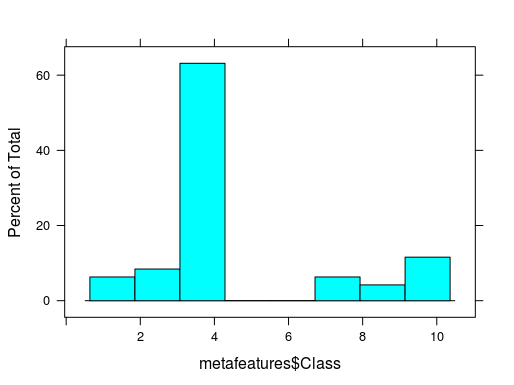
\includegraphics[width=0.9\textwidth]{khist}
	\caption{Ιστόγραμμα υπερ-παραμέτρου κ για βελτιστοποίηση με \gls{TPE}.}	
	\label{fig:khist}
\end{minipage}
	\begin{minipage}{0.48\textwidth}
		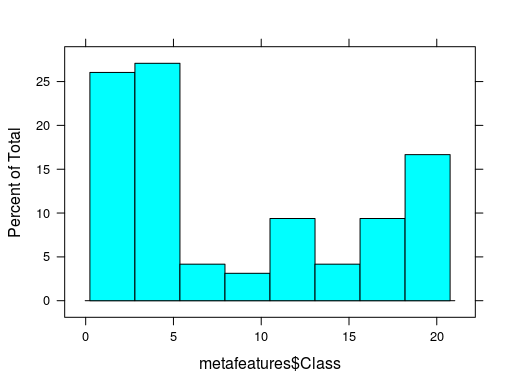
\includegraphics[width=0.9\textwidth]{kgridhist}
		\caption{Ιστόγραμμα υπερ-παραμέτρου κ για βελτιστοποίηση με πλεγματική αναζήτηση.}	
		\label{fig:kgridhist}
	\end{minipage}
\end{figure}

Παρατηρούμε πως στο σχήμα \ref{fig:khist} το δείγμα μας είναι συγκεντρωμένο στην τιμή 4, με αποτέλεσμα οι υπόλοιπες να είναι εξωκείμενες. Καθώς η ιδιότητα αυτή καθιστά την εκπαίδευση του \gls{HPP} μοντέλου ιδιαίτερη αναπτύχθηκε μία νέα τεχνική, αυτή της πρόβλεψης με χρήση General-inflated Generalized Poisson μοντέλου, την οποία αναλύουμε στην επόμενη ενότητα. Επίσης, στην Ενότητα \ref{section:HPPk} θα εκπαιδεύσουμε ένα μοντέλο παλινδρόμησης με χρήση των τιμών που προέκυψαν από την πλεγματική αναζήτηση, θεωρώντας το κ συνεχές. 

\subsubsection{Πρόβλεψη με χρήση General-inflated Generalized Poisson μοντέλου} \label{section:GIGP}
Η στατιστική ανάλυση θετικών και ακεραίων τιμών, οι οποίες στη βιβλιογραφία περιγράφονται ως μεταβλητές πλήθους (count variables) γίνεται με χρήση κατανομών όπως η Poisson και η αρνητική διωνυμική. Καθώς οι κατανομές αυτές περιέχουν ένα μικρό πλήθος παραμέτρων έχει διαπιστωθεί πως δεν είναι επαρκείς για τη περιγραφή της διακύμανσης σε πραγματικά σετ δεδομένων. Τα Γενικευμένα μοντέλα \citep{Neld:Wedd:1972} εισήχθησαν προκειμένου να αντιμετωπιστεί αυτό το πρόβλημα με χρήση βαρών σε μεταβλητές προβλέπτες. Ενώ λοιπόν το μοντέλο Poisson περιγράφεται από τη συνάρτηση μάζας πιθανότητας:

\begin{equation}
 p(\kappa \mid \lambda) = \frac{\lambda^\kappa}{\kappa!} e^{-\lambda}
 \label{eq:poisson}
\end{equation}   

όπου $\kappa$ το ζητούμενο σημείο και $\lambda$ η μέση τιμή της κατανομής, το Γενικευμένο μοντέλο διατυπώνεται ως εξής:

\begin{equation}
 p(\kappa \mid \lambda, \alpha) = \frac{\mu_k}{1+\alpha \mu_k} ^k \frac{1+\alpha k}{k!}^{k-1} e^{\frac{-\mu_k(1+\alpha y_k)}{1+\alpha \mu_k}}
 \label{eq:gpoisson}
\end{equation}

όπου $\mu_k(x_k) = e^{\sum_{}^{} x_{ij} \beta_j}$, με $x_{ij}$ τις τιμές των μεταβλητών προβλεπτών και $\beta$ τα βάρη τους. Η παράμετρος $\alpha$ ρυθμίζει την υπερ-διακύμανση (overdispersion) του μοντέλου.

Η διαπίστωση παρουσίας εκτεταμένους πλήθους μηδενικών τιμών σε πολλά πραγματικά προβλήματα οδήγησε στο σχηματισμό των zero-inflated poisson μοντέλων \citep{Lambert:1992:ZPR:149268.149270}, που προσπαθούν να διορθώσουν την υπερ-διακύμανση υπολογίζοντας ένα μοντέλο για τα μηδενικά και ένα για τις υπόλοιπες τιμές. Ο \citet{gip} γενικεύει τα μοντέλα αυτά διατυπώνοντας τη συνάρτηση πυκνότητας πιθανότητας ενός general-inflated poisson μοντέλου, δηλαδή ενός μοντέλου το οποίο μπορεί να προσαυξηθεί με κατανομές σε οποιοδήποτε σημείο συσσώρευσης τιμών, ως εξής: 
\begin{equation}
 p(\kappa \mid \lambda, \pi_i, 1 \leq i \leq m) = \begin{cases}
 \pi_i + (1-\sum_{i=1}^{m} \pi_i) p(\kappa \mid \lambda) , & \text{εάν $k=k_1, \cdots, k_m$}.\\
 (1-\sum_{i=1}^{m} \pi_i) p(\kappa \mid \lambda), & \text{εάν $k \neq k_i, 1 \leq i \leq m$}.
 \end{cases}
\end{equation}

όπου $p(\kappa \mid \lambda)$ η Poisson συνάρτηση μάζας πιθανότητας όπως αυτή ορίζεται στην Εξίσωση \ref{eq:poisson} και $\pi_i$ μία παράμετρος που ορίζει τη μάζα στο σημείο συσσώρευσης $i$ από τα συνολικά $m$.

Οι \citet{Famoye_onthe} περιγράφουν τα zero-inflated Generalized Poisson μοντέλα, ένα συνδυασμό μεθόδων για την αντιμετώπιση της υπερ-διακύμανσης και του εκτεταμένου πλήθους μηδενικών. 

Για τις ανάγκες του προβλήματος που αντιμετωπίζουμε θα ορίσουμε το General-inflated Genera\-lized Poisson μοντέλο, προκειμένου να εκμεταλλευτούμε τα μετα-χαρακτηριστικά και να αντιμετωπίσουμε την συσσώρευση τιμών στο 4. Προς αυτό το σκοπό θα συνδυάσουμε τα δύο προηγούμενα μοντέλα στην ακόλουθη συνάρτηση μάζας πιθανότητας:

\begin{equation}
 p(\kappa \mid \lambda, \phi_i, 1 \leq i \leq m) = \begin{cases}
 \phi_i + (1-\sum_{i=1}^{m} \phi_i) p(\kappa \mid \lambda, \alpha) , & \text{εάν $k=k_1, \cdots, k_m$}.\\
 (1-\sum_{i=1}^{m} \phi_i) p(\kappa \mid \lambda, \alpha), & \text{εάν $k \neq k_i, 1 \leq i \leq m$}.
 \end{cases}
\end{equation} 
 
 όπου $p(\kappa \mid \lambda, \alpha)$ η Generalized Poisson συνάρτηση μάζας πιθανότητας όπως αυτή ορίζεται στην Εξίσωση \ref{eq:gpoisson} και $\pi_i$ μία παράμετρος που ορίζει τη μάζα στο σημείο συσσώρευσης $i$ από τα συνολικά $m$.
 
 Βασισμένοι στα πειράματα των \citep{gip} και \citep{Famoye_onthe} ακολουθήσαμε την ακόλουθη διαδικασία για την προσαρμογή ενός General-inflated Generalized Poisson μοντέλου στα δεδομένα μας:
 \begin{itemize}
 	\item Προσαρμογή ενός Generalized Poisson μοντέλου για την εύρεση αρχικών τιμών για $\alpha$, $\beta$.
 	\item Προσαρμογή ενός General-inflated Poisson μοντέλου για την εύρεση των αρχικών τιμών των $\pi$.
 	\item Χρήση των αρχικών τιμών για προσαρμογή ενός General-inflated Generalized Poisson μοντέλου.
 \end{itemize}
 
 Η προσαρμογή των μοντέλων γίνεται βελτιστοποιώντας τις παραμέτρους με χρήση της τεχνικής Maximum Likelihood Estimation με αλγόριθμο αναζήτησης τη μέθοδο Nelder-Mead. Καθώς ο αλγόριθμος αυτός είναι ευαίσθητος στις αρχικές τιμές των παραμέτρων πραγματοποιήσαμε cross-validation σε ένα πλέγμα αρχικών τιμών για τα βήματα 1 και 2. Στα διάγραμματα \ref{fig:low} και \ref{fig:high} βλέπουμε τη συνάρτηση μάζας πιθανότητας του προσαρμοσμένου μοντέλου και τις πραγματικές συχνότητες των δεδομένων μας:
 
\begin{figure}[!htb]
	\begin{minipage}{0.48\textwidth}
		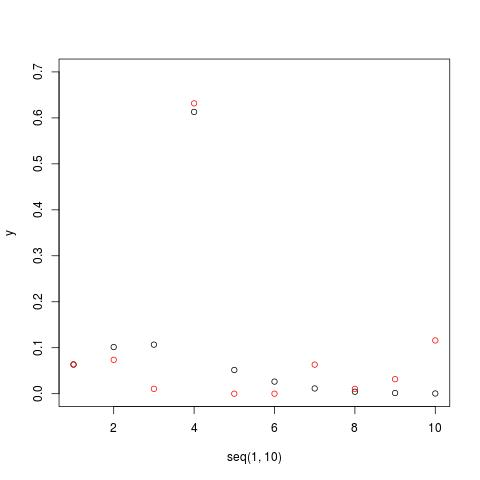
\includegraphics[width=0.9\textwidth]{gigp_low}
		\caption{Σύγκριση General-inflated Generalized Poisson συνάρτηση μάζας πιθανότητες με πραγματικές συχνότητες: Αρχικοποίηση που προσαρμόζεται καλά στο σημείο συσσώρευσης και στις χαμηλές τιμές.}	
		\label{fig:low}
	\end{minipage}
	\begin{minipage}{0.48\textwidth}
		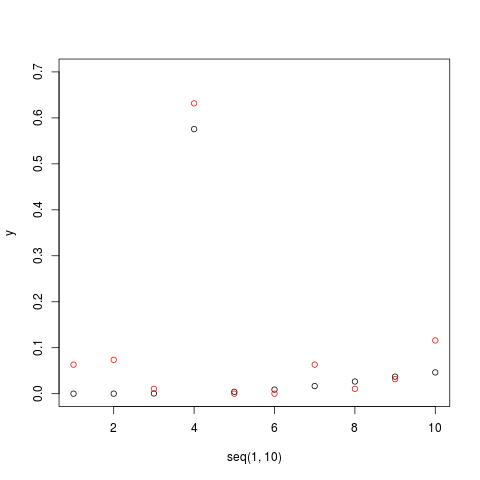
\includegraphics[width=0.9\textwidth]{gigp_high}
		\caption{Σύγκριση General-inflated Generalized Poisson συνάρτηση μάζας πιθανότητες με πραγματικές συχνότητες: Αρχικοποίηση που προσαρμόζεται καλά στο σημείο συσσώρευσης και στις υψηλές τιμές.}	
		\label{fig:high}
	\end{minipage}
\end{figure}
\FloatBarrier
\subsubsection{Εκπαίδευση μοντέλου παλινδρόμησης για κ του κ-κοντινότερου γείτονα} \label{section:HPPk}
\begin{figure}[!htb]
	\footnotesize
	\begin{center}
		\captionof{table}{Επιλογή αλγορίθμου για την υπερ-παράμετρο k του κ-κοντινότερου γείτονα}
		\begin{tabular}{ |c|c|c|c| } 
			\hline
			& Χωρίς προ-επεξεργασία & Με επιλογή χαρακτηριστικών & \pbox{20cm}{Με επιλογή χαρακτηριστικών\\ και κανονικοποίηση} \\
			\hline
			lm &  & $14 \cdot e+15$ &   \\
			\hline
			lm + log & & $7.946205 ^{*}$~\footnote{Η συνοδεία μιας μέτρησης με $^*$ υποδηλώνει ότι κρίθηκε χρήσιμο να αφαιρεθούν κάποια παραδείγματα από το σετ ελέγχου, καθώς την επηρέαζαν υπερβολικά. Αποτελεί ικανότητα του συστήματος η αναγνώριση τέτοιων παραδειγμάτων και η αποδοχή αδυναμίας εκπαίδευσης για αυτά. }& \\
			\hline
			svmRadial & $7.387213$ &$5.813214$& \\
			\hline
			svmRadial + log& $6.255705$ & $5.89$& $6.096127$\\
			\hline
			ranger + log  & $5.794678$ & 5.39141 & $5.227026$\\
			\hline
		\end{tabular}   
	\end{center}
\end{figure}

Στη συνέχεια εκπαιδεύουμε ένα μοντέλο παλινδρόμησης με χρήση του αλγορίθμου randomForest με λογαριθμικό μετασχηματισμό και εφαρμογή φιλτραρίσματος, προς-τα-εμπρός επιλογής χαρακτηριστικών και κανονικοποίησης κατά την προ-επεξεργασία.

\begin{figure}[!htb]
	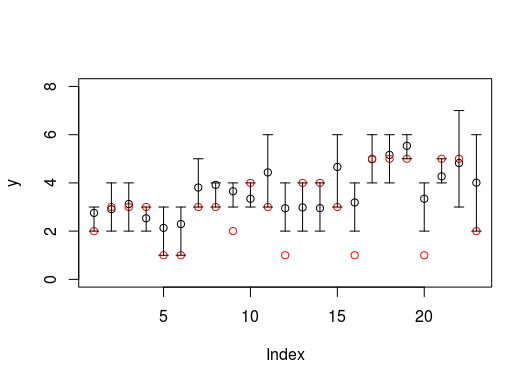
\includegraphics[width=0.9\textwidth]{test_intervals_k}
		\caption[Διάγραμμα διαστημάτων πρόβλεψης για υπερ-παράμετρο decay]{Διάγραμμα διαστημάτων πρόβλεψης για υπερ-παράμετρο k.}	
	\label{fig:high} 
\end{figure}
\FloatBarrier
\subsection{Πρόβλεψη υπερ-παραμέτρου πολυπλοκότητας για αλγόριθμo δέντρου ταξινόμησης} 
\begin{figure}[!htb]
	\footnotesize
	\begin{center}
		\captionof{table}{Επιλογή αλγορίθμου για την υπερ-παράμετρο cp του δέντρου ταξινόμησης}
		\begin{tabular}{ |c|c|c| } 
			\hline
			 & Με κανονικοποίηση & \pbox{20cm}{Με επιλογή χαρακτηριστικών\\ και κανονικοποίηση} \\
			 \hline
			lm & & $1.542080$  \\
			\hline
			lm + log && $0.78553$\\
			\hline
			svmRadial && $0.9514741$\\
			\hline
			svmRadial + log& $0.767217$& $0.768084$\\
			\hline
			ranger + log  &$0.755421$&$0.692675$\\
			\hline
			rpart + log &&$0.8007$\\
			\hline
			blackboost + log && $0.800744$ \\
			\hline
			nnet + log  && $1.3621$\\
			\hline
			cubist + log && $0.692675$ \\
			\hline
			xgbTree + log && $1.204$\\
			\hline
		\end{tabular}   
	\end{center}
\end{figure}

Στη συνέχεια εκπαιδεύουμε ένα μοντέλο παλινδρόμησης με χρήση του αλγορίθμου randomForest με λογαριθμικό μετασχηματισμό και εφαρμογή φιλτραρίσματος, προς-τα-εμπρός επιλογής χαρακτηριστικών και κανονικοποίησης κατά την προ-επεξεργασία.

\begin{figure}[!htb]
	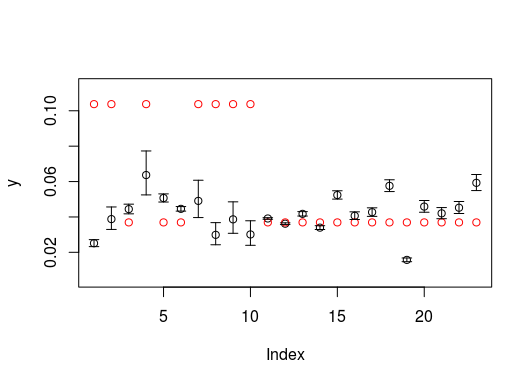
\includegraphics[width=0.9\textwidth]{test_intervals_cp}
			\caption[Διάγραμμα διαστημάτων πρόβλεψης για υπερ-παράμετρο decay]{Διάγραμμα διαστημάτων πρόβλεψης για υπερ-παράμετρο cp.}
	\label{fig:high} 
\end{figure}
\FloatBarrier
\subsection{Πρόβλεψη υπερ-παραμέτρου πλάτους πυρήνα για τον αλγόριθμο \gls{SVM}} 
\begin{figure}[!htb]
	\footnotesize
				\begin{center}
		\captionof{table}{Επιλογή αλγορίθμου για την υπερ-παράμετρο cp του δέντρου ταξινόμησης}
				\resizebox{\textwidth}{!}{ 
		\begin{tabular}{ |c|c|c|c|c|c|c| } 
			\hline
			& \pbox{20cm}{Χωρίς\\ προ-επεξεργασία} & \pbox{20cm}{Με αφαίρεση\\ ακραίων τιμών} & \pbox{20cm}{Με προς-τα-εμπρός\\ επιλογή χαρακτηριστικών} & Με φιλτράρισμα χαρακτηριστικών & \pbox{20cm}{Με φιλτράρισμα χαρακτηριστικών\\ και αφαίρεση ακραίων τιμών} &\pbox{20cm}{Με φιλτράρισμα χαρακτηριστικών\\ και αφαίρεση ακραίων τιμών\\ και κανονικοποίηση}  \\
			\hline
			lm & $15 \cdot e+13$ & $6.296997 ^*$ & $7 \cdot e+9$& $10 \cdot e+10 $ &  $69993$& $3.076596^*$     \\
			\hline
			lm + log & $4.2 \cdot e+10 ^*$ &  $4.239327$&$2.563388^*$ & Inf & $4.055437 ^*$&  $3.423858^*$\\
			\hline
			svmRadial & $2.682720$& $2.609875$ & $2.685054$ & $2.588112$ & &  $2.585245$  \\
			\hline
			svmRadial + log & $2.7075885$ & $2.702844$ & & $2.720634$ & $2.664860$ & $2.690744$   \\
			\hline
			ranger & & & & & $2.576414$& $2.671640$ \\
			\hline
			ranger + log  & &  $2.453491$ & $2.679798$& $2.6248730$& $2.696213$ & $2.530286$\\
			\hline
		\end{tabular}  }
	\end{center}
\end{figure}

Στη συνέχεια εκπαιδεύουμε ένα μοντέλο παλινδρόμησης με χρήση του αλγορίθμου randomForest με λογαριθμικό μετασχηματισμό και εφαρμογή αφαίρεσης ακραίων τιμών, φιλτραρίσματος, προς-τα-εμπρός επιλογής χαρακτηριστικών κανονικοποίησης κατά την προ-επεξεργασία.
\begin{figure}[!htb]
	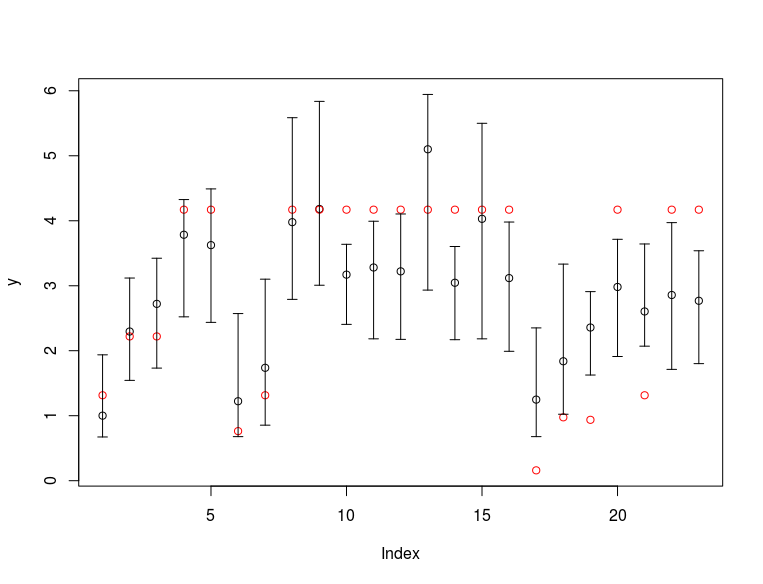
\includegraphics[width=0.9\textwidth]{test_intervals_sigma}
			\caption[Διάγραμμα διαστημάτων πρόβλεψης για υπερ-παράμετρο decay]{Διάγραμμα διαστημάτων πρόβλεψης για υπερ-παράμετρο sigma.}
	\label{fig:high} 
\end{figure}
\FloatBarrier
\subsection{Πρόβλεψη υπερ-παραμέτρου κόστους για τον αλγόριθμo \gls{SVM} }
\begin{figure}[!htb]
	\footnotesize
	\begin{center}
		\captionof{table}{Επιλογή αλγορίθμου για την υπερ-παράμετρο C του \gls{SVM}}
		\begin{tabular}{ |c|c|c|c| } 
			\hline
			& Με κανονικοποίηση & Με επιλογή χαρακτηριστικών & \pbox{20cm}{Με επιλογή χαρακτηριστικών\\ και κανονικοποίηση} \\
			\hline
			lm & $12.91$  & $12.8225$ & $12.82250$  \\
			\hline
			lm + log & $15.618852^*$ & $9.991954 ^{*}$& $9.991954^*$ \\
			\hline
			svmRadial & $10.401787$ &$10.507888$& $10.21597$\\
			\hline
			svmRadial + log& $11.136914$ & $10.676247$& $10.840548$\\
			\hline
			ranger + log  & $9.997852$ & $9.319905$ & $9.294558$\\
			\hline
		\end{tabular}   
	\end{center}
\end{figure}

Στη συνέχεια εκπαιδεύουμε ένα μοντέλο παλινδρόμησης με χρήση του αλγορίθμου randomForest με λογαριθμικό μετασχηματισμό και εφαρμογή φιλτραρίσματος, προς-τα-εμπρός επιλογής χαρακτηριστικών και κανονικοποίησης κατά την προ-επεξεργασία.

\begin{figure} [!htb]
	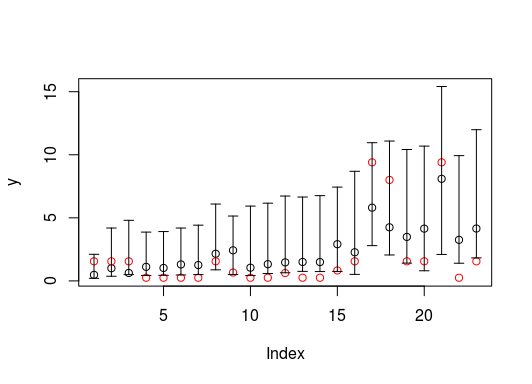
\includegraphics[width=0.9\textwidth]{test_intervals_C}
		\caption[Διάγραμμα διαστημάτων πρόβλεψης για υπερ-παράμετρο decay]{Διάγραμμα διαστημάτων πρόβλεψης για υπερ-παράμετρο C.}
	\label{fig:high} 
\end{figure}
\FloatBarrier
\subsection{Πρόβλεψη υπερ-παραμέτρου μεγέθους για τον αλγόριθμo \gls{ΤΝΝ}}
\begin{figure}[!htb]
	\footnotesize
	\begin{center}
		\captionof{table}{Επιλογή αλγορίθμου για την υπερ-παράμετρο size του \gls{ΤΝΝ}}
		\resizebox{\textwidth}{!}{ 
			\begin{tabular}{ |c|c|c|c|c|c| } 
				\hline
				& \pbox{20cm}{Χωρίς\\ προ-επεξεργασία} & \pbox{20cm}{Με αφαίρεση\\ ακραίων τιμών\\ και κανονικοποίηση} & \pbox{20cm}{Με φιλτράρισμα, \\προς τα εμπρός επιλογή χαρακτηριστικών (Boruta)\\ και αφαίρεση ακραίων τιμών} & \pbox{20cm}{Με φιλτράρισμα, \\προς τα εμπρός επιλογή χαρακτηριστικών (Boruta)\\, αφαίρεση ακραίων τιμών\\ και κανονικοποίηση} & \pbox{20cm}{Με φιλτράρισμα, \\προς τα εμπρός επιλογή χαρακτηριστικών (rfe),\\ κανονικοποίηση και αφαίρεση ακραίων τιμών} \\
			\hline
			lm + log & $4.8964 ^*$ & $4.042651$ & $2.534214$ & $2.534214$&  \\
			\hline
			svmRadial & $2.354932$& $2.358656$ & $2.164228$ & $2.113806$ & 2.208724  \\
			\hline
			svmRadial + log & $2.344243$ & $2.320754$ & $2.113830$& $2.045345$ &  2.180961  \\
			\hline
			ranger & & & $2.131324$& $2.115296$ &  \\
			\hline
			ranger + log  & $2.286583$ & $2.339490$  & $2.367264$ & $2.135809$ & \\
			\hline
			glm  &  &   &   $2.367264$ & $2.367264$ & \\
			\hline
			glm + log  &  &   &   $2.534214$ & $2.53421417$ & \\
			\hline    				
			\end{tabular}  }
		\end{center}
	\end{figure}
	
Στη συνέχεια εκπαιδεύουμε ένα μοντέλο παλινδρόμησης με χρήση του αλγορίθμου svmRadial με λογαριθμικό μετασχηματισμό και εφαρμογή αφαίρεσης ακραίων τιμών, φιλτραρίσματος, προς-τα-εμπρός επιλογής χαρακτηριστικών και κανονικοποίησης κατά την προ-επεξεργασία.
\begin{figure}[!htb]
	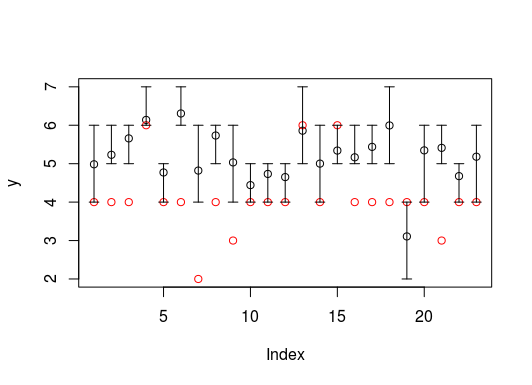
\includegraphics[width=0.9\textwidth]{test_intervals_size}
		\caption[Διάγραμμα διαστημάτων πρόβλεψης για υπερ-παράμετρο decay]{Διάγραμμα διαστημάτων πρόβλεψης για υπερ-παράμετρο size.}
	\label{fig:high} 
\end{figure}
\FloatBarrier
\subsection{Πρόβλεψη υπερ-παραμέτρου φθοράς για τον αλγόριθμo \gls{ΤΝΝ}} 
\begin{figure}[!htb]
	\footnotesize
	\begin{center}
		\captionof{table}{Επιλογή αλγορίθμου για την υπερ-παράμετρο decay του \gls{ΤΝΝ}}
		\resizebox{\textwidth}{!}{ 
			\begin{tabular}{ |c|c|c|c|c|c| } 
				\hline
				& \pbox{20cm}{Με αφαίρεση\\ ακραίων τιμών} & \pbox{20cm}{Με αφαίρεση\\ ακραίων τιμών\\κανονικοποίηση} & \pbox{20cm}{Με φιλτράρισμα, \\προς τα εμπρός επιλογή χαρακτηριστικών (Boruta)\\ και αφαίρεση ακραίων τιμών} & \pbox{20cm}{Με φιλτράρισμα, \\προς τα εμπρός επιλογή χαρακτηριστικών (Boruta)\\, αφαίρεση ακραίων τιμών\\ και κανονικοποίηση} & \pbox{20cm}{Με φιλτράρισμα, \\προς τα εμπρός επιλογή χαρακτηριστικών (rfe),\\ κανονικοποίηση και αφαίρεση ακραίων τιμών} \\
				\hline
				lm  & $1.3346 ^*$ & 1.340122  & 0.2674278  & 0.267428 &  \\
				\hline
				lm + log & $2.08406 ^*$ & 2.084079 & 0.277538& 0.277538&  \\
				\hline
				svmRadial & 0.279624 & 0.279403  & 0.270774 & 0.268606  & 0.267425   \\
				\hline
				svmRadial + log & 0.252120  & 0.253401 & 0.251316 & 0.252016  & 0.255515   \\
				\hline
				ranger & 0.276386 & 0.285601 & 0.244 & 0.247057  &  \\
				\hline
				ranger + log  & 0.250204 &  0.248379 & 0.24289  & 0.240159  & \\
				\hline    				
			\end{tabular}  }
		\end{center}
	\end{figure}
	
Στη συνέχεια εκπαιδεύουμε ένα μοντέλο παλινδρόμησης με χρήση του αλγορίθμου randomforest με λογαριθμικό μετασχηματισμό και εφαρμογή αφαίρεσης ακραίων τιμών, φιλτραρίσματος, προς-τα-εμπρός επιλογής χαρακτηριστικών και κανονικοποίησης κατά την προ-επεξεργασία.

\begin{figure}[!htb]
	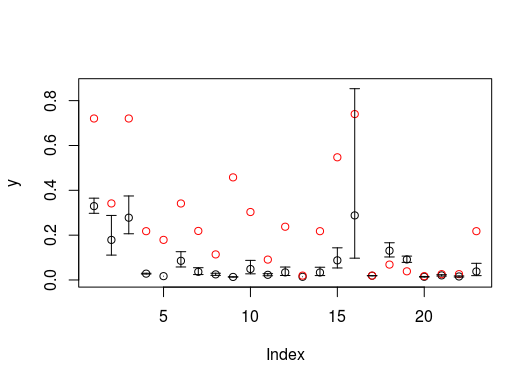
\includegraphics[width=0.9\textwidth]{test_intervals_decay}
	\caption[Διάγραμμα διαστημάτων πρόβλεψης για υπερ-παράμετρο decay]{Διάγραμμα διαστημάτων πρόβλεψης για υπερ-παράμετρο decay.}	
	\label{fig:high} 
\end{figure}
\FloatBarrier

\paragraph{Συμπεράσματα}
Τα μοντέλα HPP που εκπαιδεύσαμε απέχουν κατά πολύ από το να προβλέπουν επακριβώς τις υπερ-παραμέτρους. Το γεγονός αυτό μάλλον οφείλεται στα μετα-χαρακτη\-ρι\-στικά και συγκεκριμένα την αδυναμία τους να περιγράψουν τις συναρτήσεις-στόχους που θέσαμε. Είναι γεγονός πως δεν είμαστε βέβαιοι για την επιτευξιμότητα της πρόβλεψης υπερ-παραμέτρων, τα πειράματά μας ωστόσο δεν απορρίπτουν την ύπαρξη κάποια συσχέτισης μεταξύ αυτών και των μετα-χαρακτηριστικών.

Η προσθήκη των διαστημάτων πρόβλεψης αποδεικνύεται ότι αναιρεί την αδυναμία των μοντέλων HPP, καθώς η βέλτιστη τιμή βρίσκεται σχεδόν πάντα μέσα στο διάστημα πρόβλεψης, προσδίδοντας βαρύτητα στην αξιολόγηση του ensemble, η οποία ακολουθεί.  
\section{Αξιολόγηση της τεχνικής σχηματισμού ensemble με προς τα εμπρός επιλογή μοντέλων} \label{section:tensemble}
H αξιολόγηση της τεχνικής ensemble που χρησιμοποιήσαμε επιχειρεί να επιβεβαιώσει δύο προσδοκίες:
\begin{itemize}
	\item Ο ensemble παρουσιάζει τουλάχιστον το ίδιο καλή απόδοση με το καλύτερο μοντέλο, το οποίο βρίσκεται στην αποθήκη βελτιστοποιημένων μοντέλων. Προς αυτό το σκοπό θα συγκρίνουμε την απόδοση του ensemble με αυτήν του εκάστοτε βέλτιστου μοντέλου με δύο τεχνικές: στατιστικά τεστ υπόθεσης και διαγράμματα προφίλ απόδοσης.
	\item Ο ensemble προσθέτει μοντέλα με το βέλτιστο τρόπο. Ουσιαστικά θέλουμε να επιβεβαιώσουμε τη σωστή λειτουργία του ensemble, δηλαδή ότι σε κάθε επανάληψη έχουμε είτε σταθερή είτε βελτιωμένη απόδοση.
\end{itemize}

Για τα πειράματά μας εκπαιδεύουμε τα μοντέλα στο $80\%$ των σετ δεδομένων και κρατάμε τα υπόλοιπα για την αξιολόγηση του ensemble, η οποία γίνεται ως εξής: εξάγονται τα μετα-χαρακτηριστικά των σετ δεδομένων, προβλέπονται οι βέλτιστες υπερ-παράμετροι για κάθε αλγόριθμο μάθησης, εκπαιδεύονται τα μοντέλα και τέλος σχηματίζεται ο ensemble. Για κάθε σετ δεδομένων καταγράφεται η απόδοση του ensemble και του βέλτιστου μοντέλου ως η ακρίβεια (accuracy) που επιτεύχθηκε με 10-fold cross-validation. 

Εφαρμόζωντας το Wilcoxon-rank sum τεστ με επίπεδο εμπιστοσύνης $95\%$ διαπιστώνουμε πως ..., καθώς το p-value ισούται με ... .

\paragraph{Διαγράμματα προφίλ απόδοσης} 	Τα διαγράμματα προφίλ απόδοσης (performance profile plots) \citep{Dolan2002} αποτελούν ένα εργαλείο αξιολόγησης και σύγκρισης της απόδοσης εργαλείων βελτιστοποίησης. Χρησιμοποιούνται σε περιπτώσεις εφαρμογής διαφορετικών τεχνικών βελτιστοποίησης σε ένα σύνολο προβλημάτων ως εναλλακτική απεικόνιση εκτενών πινάκων, μιας συνηθισμένης και προβληματικής λύσης. Το προφίλ απόδοσης είναι η αθροιστική συνάρτηση κατανομής μιας τεχνικής για μία μετρική απόδοσης.

Ως μετρική απόδοσης ορίζουμε το λόγο της απόδοσης της τρέχουσας τεχνικής προς τη μεγαλύτερη απόδοση που επιτεύχθηκε από οποιαδήποτε τεχνική για ένα συγκεκριμένο σετ δεδομένων, δηλαδή

\begin{equation}
r_{p,s}= \frac{t_{p,s}}{\max\{{t_{p,s} : s \in S}\}}    
\end{equation} 

όπου r ο λόγος απόδοσης, t η ακρίβεια, p το σετ δεδομένων και s η τεχνική.

Το διάγραμμα απεικονίζει τη τιμή
\begin{equation}
\rho_{\tau}= \frac{size\{{p \in P : r_{p,s} \leq \tau  }\}}{n_p}   
\end{equation}

όπου $n_p$ το πλήθος των σετ δεδομένων. Η τιμή αυτή εκφράζει την πιθανότητα μία τεχνική να βρίσκεται σε απόσταση $\tau$ από τον καλύτερο λόγο απόδοσης.  Επομένως το σημείο $\tau = 1$ εκφράζει τη πιθανότητα μία τεχνική να είναι η βέλτιστη.


\begin{figure}[!htb]
	\begin{center}
		\caption[Διάγραμμα προφίλ απόδοσης για τη σύγκριση του ensemble με το βέλτιστο μοντέλο]{Διάγραμμα προφίλ απόδοσης για τη σύγκριση του ensemble με το βέλτιστο μοντέλο: Παρατηρούμε πως }
	\end{center}
\end{figure}

\begin{figure}[!htb]
	\begin{center}
		\caption[Διάγραμμα εξέλιξης ensemble για το σετ δεδομένων (όνομα)]{Διάγραμμα εξέλιξης ensemble για το σετ δεδομένων (όνομα): Παρατηρούμε πως σε κάθε επανάληψη η απόδοση του ensemble είτε μειώνεται είτε παραμένει σταθερή. }
	\end{center}
\end{figure} 	

\paragraph{Συμπεράσματα}
\section{Αξιολόγηση συστήματος Automated Data Scientist}\label{section:eval_system}
Η αξιολόγηση του Automated Data Scientist στοχεύει να αποδείξει ότι το σύστημα που έχουμε σχεδιάσει έχει απόδοση συγκρίσιμη με τεχνικές της σύγχρονης βιβλιογραφίας. Καθώς η ουσιαστική πρωτοτυπία του συστήματος βρίσκεται στον τρόπο με τον οποίο γίνεται η βελτιστοποίηση των υπερ-παρα\-μέ\-τρων για τα μοντέλα μηχανικής μάθησης που χρησιμοποιούμε θα συγκρίνουμε το σύστημά μας με δύο τεχνικές βελτιστοποίησης:
\begin{itemize}
	\item πλεγματική αναζήτηση. Πρόκειται για τη συνηθέστερη τεχνική αναζήτησης υπερ\-παραμέτρων μέχρι και σήμερα.
	\item Tree Parzen Estimator. Η τεχνική αυτή, που έχει περιγραφεί στην ενότητα \ref{section:SMBO} αποτελεί state of the art στο χώρο του AutoML.
\end{itemize}

Η διεξαγωγή των πειραμάτων ακολουθεί τη λογική της ενότητας \ref{section:tensemble}. Έχουμε πραγματοποιήσει 6 διαφορετικά πειράματα: ένα για το συνολικό σύστημα και ένα χρησιμοποιώντας στον ensemble μοντέλα μόνο ενός αλγορίθμου μάθησης. Οι υποπεριπτώσεις αυτές λαμβάνονται υπόψη για τη σύγκριση των τριών τεχνικών επί ίσοις όροις. Φυσικά εμείς ενδιαφερόμαστε περισσότερο για την απόδειξη υπεροχής του συνολικού συστήματος.  

[Ακολουθούν τα διαγράμματα προφίλ απόδοσης]
	
\paragraph{Συμπεράσματα}